%%==================================================
%% chapter01.tex for BIT Master Thesis
%% modified by pinren lu
%% version: 0.1
%% last update: Dec 25th, 2016
%%==================================================
% 相关工作

% 1. 文本生成技术
% 2. 大语言模型生成技术
% 3. 文本分类技术
% 4. 大语言模型文本探测技术
% 5. 本章小结

\chapter{相关工作}
\label{chap:related works}

\section{文本生成技术}
\label{sec:rw-lm}

在当前自然语言处理领域,主流的大语言模型普遍基于 Transformer 框架 \cite{transformer}。自2017年提出以来,该架构因其卓越的并行处理能力和对长距离依赖的建模能力而迅速成为研究的热点。Transformer 通过自注意力机制有效地捕捉输入序列中各部分之间的关系,从而显著提升了在处理大规模文本数据时的训练效率和表达能力。诸如 BERT 和 GPT 系列等知名模型均依托该框架,在多种语言任务中展现出卓越的性能。因此,深入探讨 Transformer 的结构与原理,不仅有助于理解当前大语言模型成功的原因,也为未来研究奠定了重要的理论基础。

Transformer 是 Google 于2017年提出的一种基于自注意力机制的神经网络模型,专为处理序列到序列(Seq2Seq)任务而设计,广泛应用于各种自然语言处理任务。该模型利用自注意力机制来处理输入序列中的关联性,能够有效捕捉长距离依赖关系,而无需依赖循环神经网络或卷积神经网络。此外,Transformer 可以并行处理输入序列中的不同位置,因此在训练和推理过程中,特别是在处理长序列时,展现出更高的效率。

\begin{figure}[htb]
	\centering
	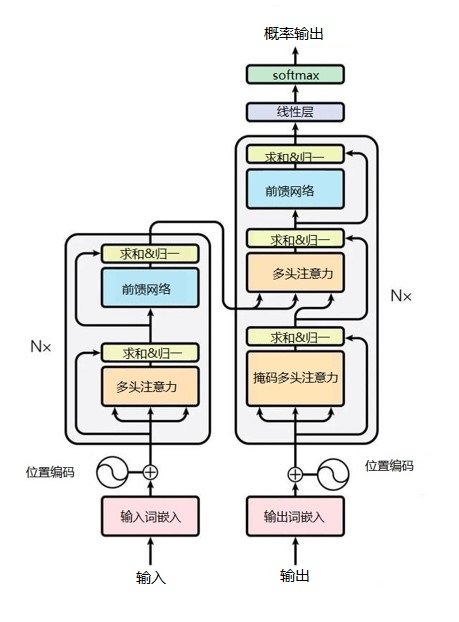
\includegraphics[scale = 0.8]{figures/Transformer2}
	\caption{Transformer 模型结构 \cite{transformer}}
	\label{fig:Transformer2}
\end{figure}

\subsection{编码器-解码器结构}

(1) 编码器

编码器由 \(N=6\) 个相同的 TransformerEncoderLayer 层构成。每个 TransformerEncoderLayer 层可分为两个子层。第一个子层实现了多头自注意力机制,而第二个子层则是一个简单的全连接前馈网络。每个子层后均接有残差连接,随后对经过残差连接的输出进行层归一化。简而言之,每个子层的输出向量可表示为 \(\text{LayerNormal}(x + \text{Sublayer}(x))\),其中 \(\text{Sublayer}(x)\) 表示该子层所实现的功能。为了确保残差连接的维度相等并便于计算,模型中所有子层及嵌入层的输出向量均设定为 \(d_{\text{model}} = 512\)。

(2) 解码器

解码器同样由 \(N=6\) 个相同的 TransformerDecoderLayer 层组成。每个 TransformerDecoderLayer 层包含三个子层。其中两个子层的结构与编码器层中的子层大致相似,而第三个子层则接收编码器堆栈的输出及解码器层前一个多头注意力子层的输出,并在该子层内执行多头注意力操作。与编码器层的子层结构相似,解码器层的每个子层后也接有残差连接,随后对经过残差连接的输出进行层归一化。此外,本研究对解码器结构中的自注意力子层进行了修改,加入了位置掩码,以防止从前面某个位置获取后面位置的信息。此位置掩码结合位置偏移的设计,确保序列中位置 \(i\) 的元素的预测仅能基于序列中小于 \(i\) 的所有内容。

\subsection{注意力机制}

在 Transformer 中,定义注意力函数为输入为查询和一组键值,然后进行输出的函数,在此之中查询(Query, Q)、键(Key, K)、值(Value, V)和输出都是向量。在注意力函数中,简单地讲,输出实质上是值的加权和。此其中对于每个值的权重由权重相应的键以及查询计算得出。

(1) 缩放点积注意力

在 Transformer 论文中所采用的注意力机制为缩放点积注意力。该机制的输入由查询、键和值组成,其中查询和键的维度均为 \(d_k\),而值的维度为 \(d_v\)。在缩放点积注意力中,我们首先计算查询与所有键向量之间的点积,并随后将这些结果除以 \(\sqrt{d_k}\)。接着,通过 softmax 函数对这些归一化后的向量进行处理,以计算每个值的权重。具体的过程如图 \ref{fig:DotAtt} 所示。

\begin{figure}[htbp]
	\centering
	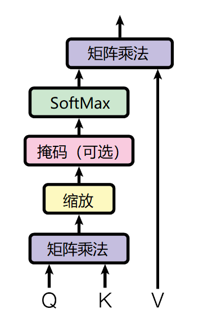
\includegraphics[scale = 0.8]{figures/DotAtt}
	\caption{缩放点积注意力 \cite{transformer}}
	\label{fig:DotAtt}
\end{figure}

在实际应用中,对于一组待处理的注意力查询,应将这些查询同时进行计算,并将其封装为一个矩阵 \(Q\)。类似地,键和值也被封装为矩阵 \(K\) 和 \(V\)。通过这种方式,计算过程可以通过矩阵乘法进行优化。因此,注意力函数的输出矩阵可以表示为:
\begin{equation}
\text{Attention}(Q,K,V) = \text{softmax}(\frac{QK^T}{\sqrt{d_k}})V
\label{eq3.1}
\end{equation}

(2) 多头注意力

实际上,如果将键、值和查询统一设定为 \(d_{\text{model}}\) 维度,反而可能导致模型性能下降,相较于将查询、键和值分别投影至 \(d_k\)、\(d_k\) 和 \(d_v\) 维度进行不同的线性变换。在此基础上,注意力函数在每个查询、键和值的投影向量上并行执行,从而生成 \(d_v\) 维的输出值。随后,将这些 \(d_v\) 维的输出值进行连接,并再次进行线性投影,以生成最终输出。具体过程如图 \ref{fig:MultiheadAtt} 所示。

\begin{figure}[htbp]
	\centering
	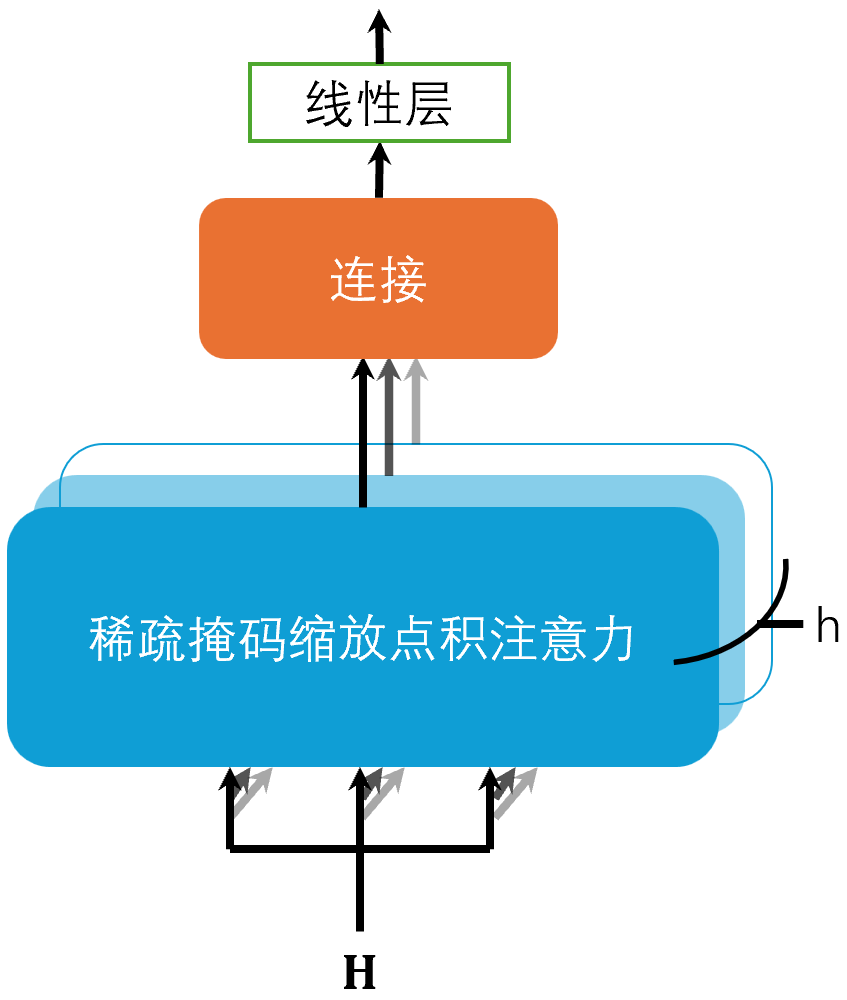
\includegraphics[scale = 0.8]{figures/MultiheadAtt}
	\caption{多头注意力 \cite{transformer}}
	\label{fig:MultiheadAtt}
\end{figure}

多头注意力的主要优势在于其能够同时关注来自不同位置的信息。相较之下,单一注意力头的使用会导致信息的平均化,从而抑制这一特性。
\begin{equation}
\text{MultiHead}(Q, K, V) = \text{Concat}(\text{head}_1, ..., \text{head}_h)W^O
\label{eq3.2}
\end{equation}
\begin{equation}
\text{head}_i = \text{Attention}(QW_i^Q, KW_i^K, VW_i^V)
\label{eq3.3}
\end{equation}
在上述公式中,投影操作涉及的参数矩阵包括 \(W_i^Q \in \mathbb{R}^{d_{\text{model}}}\)、\(W_i^K \in \mathbb{R}^{d_{\text{model}} \times d_k}\)、\(W_i^V \in \mathbb{R}^{d_{\text{model}} \times d_v}\) 以及 \(W^O \in \mathbb{R}^{hd_v \times d_{\text{model}}}\)。

在 Transformer 架构中,采用了 \(h = 8\) 个并行的注意力层或头。对于每个注意力头,设定其维度为 \(d_k = d_v = d_{\text{model}} / h = 64\)。由于每个头的维度被缩减,因此整体计算成本与具有全维度的单头注意力相当。

\subsection{位置前馈网络}

除了注意力子层外,编码器和解码器的每一层均包含一个全连接的前馈网络,该网络在每个位置上均以相同方式应用。该网络包括两个线性变换,并在其间引入一个线性整流单元(ReLU)激活函数。具体表达式为:
\begin{equation}
\text{FFN}(x) = \max(0, xW_1 + b_1)W_2 + b_2
\label{eq3.4}
\end{equation}

尽管在不同位置上应用的线性变换相同,但在层与层之间所使用的参数却是各异的。可以将其视作两个内核大小为 \(1\) 的卷积操作。输入和输出的维度均为 \(d_{\text{model}} = 512\),而内部层的维度为 \(d_{ff} = 2048\)。

\subsection{嵌入层与 Softmax 函数}

与其他序列转换模型相似,Transformer 采用学习嵌入技术,将输入序列和输出序列中的词汇映射为维度为 \(d_{\text{model}}\) 的向量。此外,模型还利用常规的学习线性变换及 Softmax 函数,将解码器的输出转化为对下一个词汇的预测概率。在我们的模型中,两个嵌入层与预 Softmax 线性变换之间共享相同的权重矩阵。在嵌入层中,这些权重会乘以因子 \(\sqrt{d_{\text{model}}}\)。此外,也存在将 log-softmax 函数替代 Softmax 函数的做法。

\subsection{位置编码}

由于 Transformer 模型不采用递归或卷积结构,为了使模型能够有效利用序列的顺序信息,必须引入某种形式的标记在序列中相对或绝对位置的信息。因此,我们在编码器和解码器堆栈的输入嵌入中添加了“位置编码”。位置编码的维度与嵌入相同,即 \(d_{\text{model}}\),从而可以将两者直接相加。位置编码的形式多种多样,既可以通过模型学习得到,也可以通过预定义的公式计算得出。

在 Transformer 中,采用了不同频率的正弦和余弦函数来生成位置编码,具体表达式为:
\begin{equation}
\begin{aligned}
\text{PE}(pos,2i) &= \sin \left ( \frac{pos}{10000^{2i/d_{\text{model}}}} \right ) \\
\text{PE}(pos,2i+1) &= \cos \left ( \frac{pos}{10000^{2i/d_{\text{model}}}} \right )
\end{aligned}
\label{eq3.5}
\end{equation}
其中 \(pos\) 表示位置,\(i\) 表示维度。换言之,位置编码的每个维度对应于一条正弦曲线,其波长形成从 \(2\pi\) 到 \(10000 \cdot 2\pi\) 的几何级数。选择这种函数的原因在于我们假设它能够使模型更容易地学习通过相对位置进行计算,因为对于任何固定的偏移量 \(k\),\(\text{PE}_{pos+k}\) 可以表示为 \(\text{PE}_{pos}\) 的线性函数。

\subsection{线性层}

在数据经过 log-softmax 函数处理后,将通过一层线性层将维度为 \(d_{\text{model}}\) 的向量转换为一个维度等于词汇表大小的向量,该向量用于表示对下一个预测词汇的概率分布。

\section{预训练语言模型技术}

近年来,自然语言处理(Natural Language Processing, NLP)领域经历了显著的进展,其中预训练语言模型(Pre-trained Language Models, PLMs)的研究为该领域的发展提供了重要支持。预训练语言模型的核心思想是首先在大规模数据集上对深度神经网络进行预训练,以获得模型参数,随后利用这些经过训练的模型来执行多种具体的下游任务,从而避免从零开始训练模型并减少对标注数据的依赖。与预训练语言模型相关的早期研究可以追溯到 NNLM \cite{NNLM} 和 word2Vec \cite{mikolov2013efficientestimationwordrepresentations}。2017 年,Vaswani 等人 \cite{transformer} 提出了 Transformer 架构,这一架构的引入显著提升了多种 NLP 任务的性能,使 Transformer 成为众多预训练语言模型的基础。在基于 Transformer 的编码器架构中,Radford 等人 \cite{gpt} 提出了 GPT 模型,该模型真正实现了预训练-微调的框架,避免了将词嵌入从模型中提取的过程,而是直接在下游任务中对预训练模型进行微调。不同的任务可以采用不同的输入或对输出层进行调整,使下游任务更紧密地结合上游的预训练模型。目前,GPT 模型的应用取得了显著成功,各种大型 GPT 模型层出不穷,为 NLP 等领域注入了新的活力。同时,Devlin 等人 \cite{devlin_bert_2019} 基于 Transformer 的编码器提出了 BERT 模型,成为目前 NLP 中应用最广泛的预训练模型之一。BERT 采用了一种掩码语言模型(Masked Language Model, MLM)的方法,通过随机掩盖输入文本中的某些词元,并利用上下文信息进行预测,从而实现对数据语义关系的提取。继 GPT 和 BERT 之后,研究人员还提出了 XLNet \cite{XLNet}、RoBERTa \cite{liu_roberta_2019}、DeBERTa \cite{he_deberta_2021}、ERNIE \cite{sun2019ernieenhancedrepresentationknowledge}、T5 \cite{T5} 和 BART \cite{lewis-etal-2020-bart} 等多种预训练语言模型。本节将介绍本文所采用的 RoBERTa 和 DeBERTa 模型的基础预训练语言模型 BERT。

% 写写 BERT 吧
BERT(Bidirectional Encoder Representations from Transformers)\cite{devlin_bert_2019} 是由 Google AI 研究院于 2018 年 10 月提出的一种预训练模型。该模型在机器阅读理解的顶级基准测试 SQuAD1.1 \cite{rajpurkar2016squad100000questionsmachine} 中展现了卓越的性能:在所有两个评估指标上均显著超越了人类表现,并在 11 项不同的 NLP 测试中创造了最新的状态-of-the-art(SOTA)成绩。其中,GLUE 基准 \cite{wang2019gluemultitaskbenchmarkanalysis} 的得分提升至 80.4\%(绝对改进 7.6\%),而 MultiNLI 数据集 \cite{williams2018broadcoveragechallengecorpussentencemultinli} 的准确率达到 86.7\%(绝对改进 5.6\%),标志着这一模型在自然语言处理领域的里程碑式成就。BERT 在 Transformer 架构的基础上引入了预训练与微调的策略,使得模型能够在预训练阶段学习通用的语言表示,并在特定任务中进行微调,从而显著提高了模型的适应性与性能。因此,尽管 BERT 并非首个预训练模型,但在预训练模型的发展历程中,其重要性不容忽视,具有里程碑式的意义。

\subsection{BERT 结构}

BERT 在 Transformer 的基础上并未进行大量改进,而是采用了 Transformer 编码器的结构作为其核心架构。其总体结构如图 \ref{fig:BERT} 所示,多个 Transformer 编码器层逐层堆叠构成了 BERT 的整体框架。在原始论文中,作者分别构建了两种 BERT 模型,采用了 12 层和 24 层的 Transformer 编码器,分别对应于 110M 和 340M 的总参数量。

\begin{figure}[htb]
	\centering
	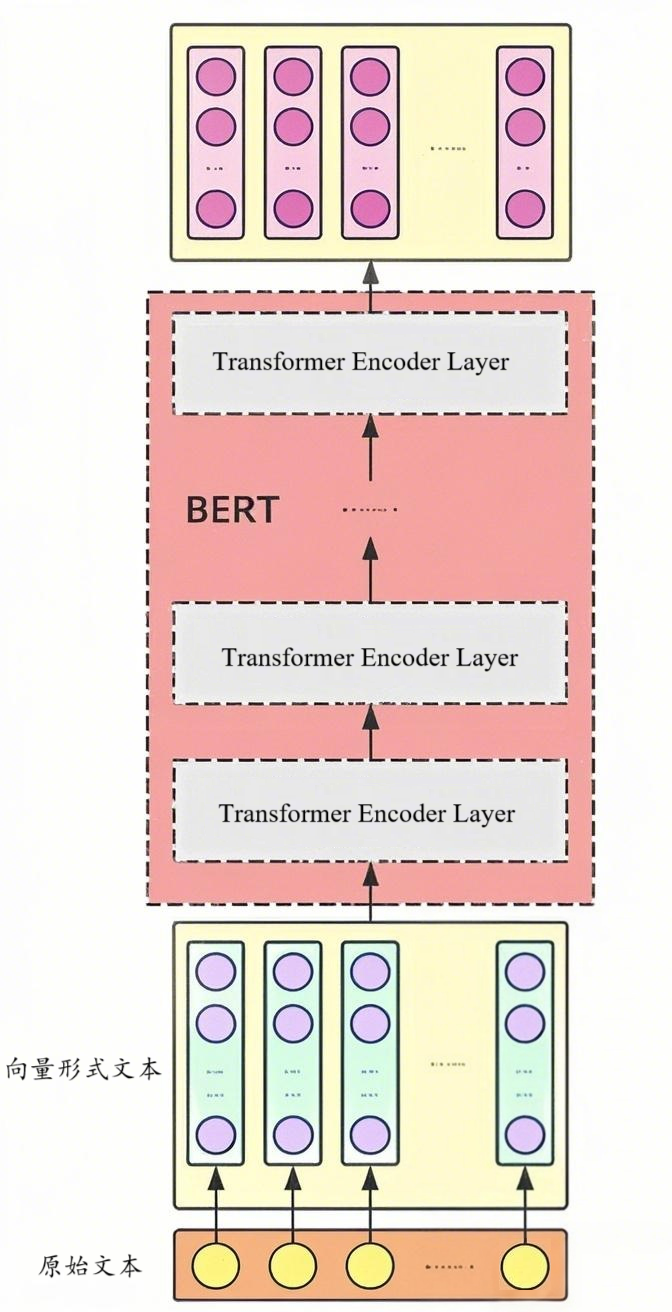
\includegraphics[scale = 0.5]{figures/bert.png}
	\caption{BERT 架构图 \cite{devlin_bert_2019}}
	\label{fig:BERT}
\end{figure}

\subsection{嵌入}

对于 BERT 而言,其在嵌入(Embedding)方面的显著改进是一个关键创新。为了使 BERT 能够有效处理多种下游任务,其输入表示能够清晰地区分单个句子和句子对(例如,〈问题, 答案〉)在同一词元序列中。在本研究中,“句子”可以被理解为任意跨度的连续文本,而非严格意义上的自然语言句子。“序列”则是指输入到 BERT 的词元序列,这可以是单个句子,也可以是多个句子组合而成。

在 BERT 中,采用了具有 30,000 个词元的 WordPiece 嵌入机制。每个序列的首个标记始终是一个特殊的分类标记([CLS]),其对应的最终隐藏状态被用作分类任务的聚合序列表示。该标记的最终向量可视为整句话的语义表示,进而用于下游的分类任务等。由于该标记本身缺乏明显的语义信息,它能够更“公平”地整合文本中各个词的语义,从而更好地表征整句话的含义。具体而言,self-attention 机制通过文本中的其他词增强目标词的语义表示,尽管目标词自身的语义仍占主导地位。因此,在经过 BERT 的 12 层(以 BERT-base 为例)处理后,每个词的嵌入融合了所有词的信息,从而更准确地反映其语义。在 BERT 的执行过程中,句子对被打包为一个单一的序列。在这种情况下,有两种方式用于区分句子。首先,通过一个特殊标记([SEP])将它们分开。其次,BERT 会将学习到的嵌入添加到每个词元中,以指示其属于句子 A 还是句子 B。

\begin{figure}[htb]
	\centering
	\includegraphics[width=0.9\linewidth]{figures/bert_Input_Embeddings.jpg}
	\caption{BERT 嵌入(Embedding)示意图 \cite{devlin_bert_2019}}
	\label{fig:BERT-embedding}
\end{figure}

对于每个给定的词元,其输入表示(input representation)是通过对相应的词元(token)、段落(segment)和位置(position)嵌入进行加和来构建的。该结构的可视化展示见图 \ref{fig:BERT-embedding}。

\subsection{预训练与微调}

BERT 研究的主要贡献在于其二阶段训练过程的有效推广,该过程分为预训练(pretraining)和微调(finetuning)两个阶段,训练流程的示意图如图 \ref{fig:BERT-OverAll} 所示。在预训练阶段,BERT 通过大规模的无标注文本数据学习语言的深层次表示,采用了带掩码的语言模型(Masked Language Model, MLM)和下一句预测(Next Sentence Prediction, NSP)两种任务,从而使模型能够理解上下文的双向信息。在微调阶段,BERT 通过在少量标注数据上进行训练,能够针对特定任务进行调整,进而高效适应多种自然语言处理任务,如文本分类、问答系统和命名实体识别等。

\begin{figure}[htb]
	\centering
	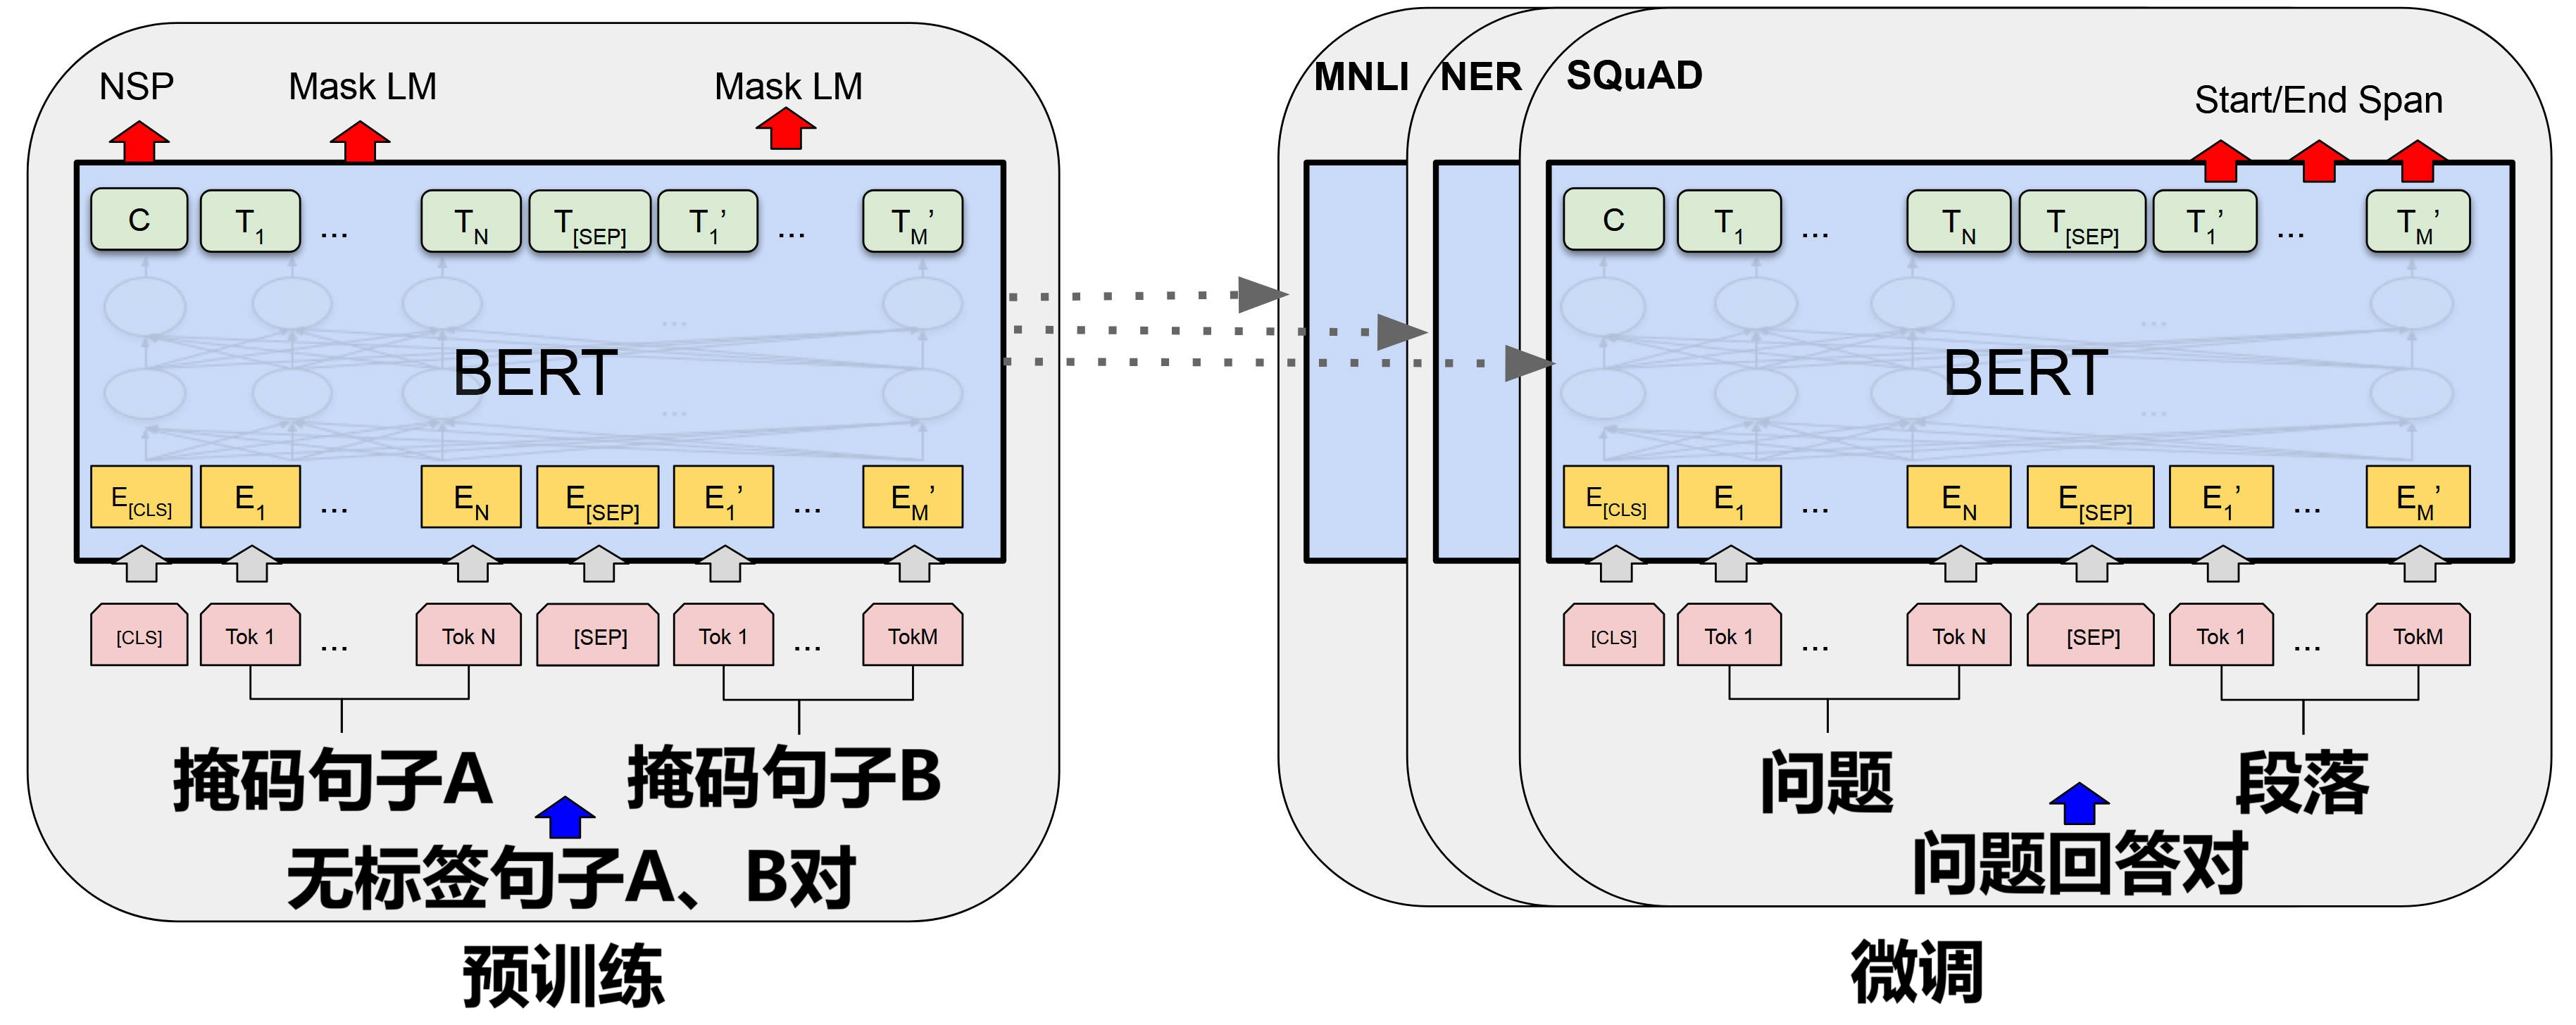
\includegraphics[width=0.9\linewidth]{figures/BERT_Overall.jpg}
	\caption{BERT 训练过程示意图 \cite{devlin_bert_2019}}
	\label{fig:BERT-OverAll}
\end{figure}

这种预训练-微调的二阶段训练范式显著提高了模型在多种自然语言处理(NLP)任务上的性能,标志着该领域的一次重要变革。BERT 的成功激励了大量基于 Transformer 架构的预训练模型的后续研发,例如本文将使用的 RoBERTa 和 DeBERTa,以及其他在 BERT 模型基础上进行改进的模型。这些模型在不同任务中展现出更高的效率和准确性。通过这些创新,BERT 不仅推动了学术界对预训练模型的深入研究,也促进了工业界在实际应用中的广泛采用。

\section{AI 生成文本检测技术}
\label{sec:llmdetect}

大型语言模型(LLMs)的迅速发展促使对检测 AI 生成文本的方法进行深入研究。在 ChatGPT 发布之前,GLTR \cite{gehrmann_gltr_2019} 作为一种文本检测工具,通过一系列统计分析技术识别由不同采样策略生成的文本特征。GLTR 有效地将人类对生成文本的检测准确率从 54\% 提升至 72\%,彰显了其在帮助非专业人士区分人类与机器生成内容方面的实用性。

另一个重要的贡献是人类 ChatGPT 比较语料库 \cite{guo_how_2023}(HC3),该语料库是在 ChatGPT 发布后开发的。HC3 数据集包含来自人类专家与 ChatGPT 的数万个响应,涵盖金融、医学和法律等多个领域。这一数据集使得对 ChatGPT 的响应与人类输出进行全面评估成为可能,从而揭示了 LLMs 的能力与局限性。此外,HC3 还促进了检测系统的发展,旨在识别文本是由 ChatGPT 还是人类生成的。

LLM-Detector \cite{wang_llm-detector_2024} 针对现有人工智能生成文本检测模型所面临的挑战进行了研究,这些模型通常因领域内过拟合而在领域外表现不佳。该研究通过收集人类专家和多种大语言模型的回复,基于大型语言模型提出了一种新颖的检测方法,利用指令调优来增强文档级和句子级的检测能力。实验结果表明,该方法在性能上显著优于基线方案,展现出强大的泛化能力。

SeqXGPT \cite{wang_seqxgpt_2023} 通过构建一个包含大语言模型生成句子与人类写作内容的数据集,引入了句子级检测挑战。该方法利用来自白盒 LLMs 的对数概率列表,结合卷积网络和自注意力机制以提高检测准确性。结果显示,SeqXGPT 在句子和文档级检测任务中均优于现有方法,进一步强调了有效检测机制的必要性。

针对人工智能生成文本来源追踪的问题 \cite{li_origin_2023},已有研究提出了一种创新的算法,旨在检测和追踪人工智能生成的内容。该方法通过对比特征有效区分由不同模型生成的文本,能够在白盒和黑盒环境中均发挥作用。研究结果突显了人工智能部署所带来的伦理影响,以及追踪生成文本来源机制的重要性,为关于人工智能系统问责制的持续讨论提供了重要的理论支持。

然而,现有的方法 \cite{gehrmann_gltr_2019, guo_how_2023, wang_llm-detector_2024, wang_seqxgpt_2023} 尚未满足我们对文本来源于特定大型语言模型的检测需求。大多数研究在分类任务上表现较为粗糙,仅能识别文本是由人类还是机器生成,无法进一步确定文本的具体来源。尽管少部分研究 \cite{li_origin_2023} 实现了识别文本来源于特定大型语言模型的目标,但其实现方式依赖于白盒测试,必须获取与待检测模型一致或相似的模型生成的特征向量才能进行判断。在当前大多数大型语言模型均为闭源的环境下,这种方法几乎缺乏扩展性和可操作性。

\section{本章小结}
\label{sec:rw-conclusion}

本章回顾了当前自然语言处理领域的相关工作,重点聚焦于文本生成技术和预训练语言模型的进展。首先,我们深入分析了Transformer架构的优势,强调了其在大语言模型中的广泛应用。自2017年提出以来,Transformer因其卓越的并行处理能力和长距离依赖建模能力,迅速成为自然语言处理研究的核心。通过自注意力机制,Transformer能够有效捕捉输入序列中各个部分之间的关系,从而显著提高了模型在处理大规模文本数据时的训练效率和表达能力。

随后,我们详细讨论了BERT模型的结构及其在预训练和微调过程中的创新。BERT不仅在机器阅读理解等多个任务中取得了显著的性能提升,还引入了预训练-微调的二阶段训练范式,使得模型能够在预训练阶段学习通用的语言表示,而在特定任务中进行微调。这一策略极大地提升了模型的适应性和性能,标志着自然语言处理领域的一次重大变革。在预训练语言模型的讨论中,我们提及了如GPT、RoBERTa和DeBERTa等模型的相继出现,这些模型在BERT的基础上进行了不同程度的改进,进一步推动了预训练模型的研究和应用。

最后,本章探讨了AI生成文本的检测技术,介绍了多种现有方法及其在实际应用中的效果与局限性。尽管GLTR、HC3、LLM-Detector、SeqXGPT等工具在识别生成文本方面取得了一定的成效,但仍面临特定大型语言模型检测的挑战。尤其是在当前许多大型语言模型为闭源的环境下,现有方法在文本来源追踪和特定模型检测方面的适用性显得尤为重要。

综上所述,本章的讨论为理解当前技术状态及未来研究方向提供了重要视角,为本论文的研究奠定了坚实的基础。通过对Transformer架构、BERT模型及AI文本检测技术的全面回顾,我们为后续的研究和实验提供了必要的理论支持和实践指导。